% !TEX program = xelatex

\documentclass{VUMIFPSkursinis}
\usepackage{algorithmicx}
\usepackage{algorithm}
\usepackage{algpseudocode}
\usepackage{amsfonts}
\usepackage{amsmath}
\usepackage{bm}
\usepackage{caption}
\usepackage{color}
\usepackage{float}
\usepackage{graphicx}
\usepackage{listings}
\usepackage{float}
\usepackage{subfig}
\usepackage{wrapfig}
\usepackage[hidelinks]{hyperref}
\usepackage{todonotes}
\usepackage{lineno}
\usepackage{pdflscape}


% Titulinio aprašas
\university{Vilniaus universitetas}
\faculty{Matematikos ir informatikos fakultetas}
\department{}
\papertype{Programų sistemų inžinerijos modeliai ir metodai laboratorinis darbas 2}
\title{Requirements modeling}
\titleineng{Reikalavimų modeliavimas}
\status{1 course students}
\author{Matas Savickis}
\secondauthor{Vytautas Krivickas}
\thirdauthor{Šarūnas Kazimieras Buteikis}


\supervisor{Audronė Lupeikienė, M. Darbuot., Dr}
\date{Vilnius – \the\year}

% Nustatymai
% \setmainfont{Palemonas}   % Pakeisti teksto šriftą į Palemonas (turi būti įdiegtas sistemoje)
\bibliography{bibliografija}

\begin{document}
\selectlanguage{english}
\maketitle

\tableofcontents

\section{NFR type catalogue}

\begin{figure}[htbp]
	\center
	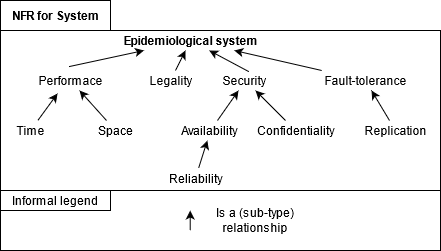
\includegraphics[scale=0.9]{img/1}
	\caption{NFR diagram} % Antraštė įterpiama po paveikslėlio
	\label{img:kurimoProcesas}
\end{figure}

	\begin{itemize}
		%\item{\textbf{Virus registration time} - to ensure quick response time system must provide quick process of registering new cases. }
		%\item{\textbf{Patient notification time} - it is important to prevent spread of virus by hastily notifying and isolating contagious patients.}
		%\item{\textbf{Holding medical records} - to ensure that the spread of the epidemic is contained and monitored, all necessary medical records related to the epidemic must be accessed via the system. }
		%\item{\textbf{Holding foreign countries data} - to check which countries are infected and are spreading the virus, the epidemiological system has to keep up-to-date epidemiological information about them.}
		\item{\textbf{Time} - System is monitoring the epidemic therefore it's processes or workflows have to be efficient time-wise.}
		\item{\textbf{Space} - since the system will contain lots of different data (e.g. person's geographical coordinates), data must be stored efficiently.}		
		\item{\textbf{Reliability} - Tracking the state of the epidemic must be ensured 24/7 to not miss any crucial data or trends.}
		\item{\textbf{Confidentiality} - epidemiological system must treat sensitive person information (e.g. received medical records) with respect to ensure systems credibility.}
		\item {\textbf{Legality} - due to the fact the the epidemiological system will deal with sensitive information, data handling must be in compliance with LT and EU data laws as well as GDPR.}
		\item{\textbf{Replication} - non sensitive data must have duplicate records stored to increase the system's fault-tolerance.}
	\end{itemize}

	\begin{landscape}
\section{Modelling of the non-functional requirements}
	\subsection{Self-isolation}
		\begin{figure}[H]
			\center
			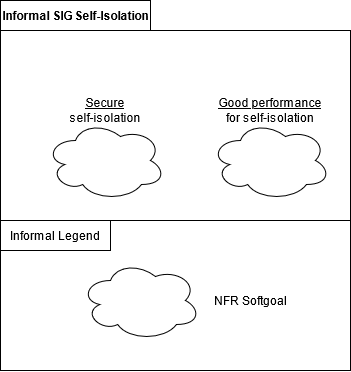
\includegraphics[scale=0.9]{img/Self-Isolation-1}
			\caption{Self Isolation - Initial Software Dependency Graph} % Antraštė įterpiama po paveikslėlio
			\label{img:kurimoProcesas}
		\end{figure}
		\begin{figure}[H]
			\center
			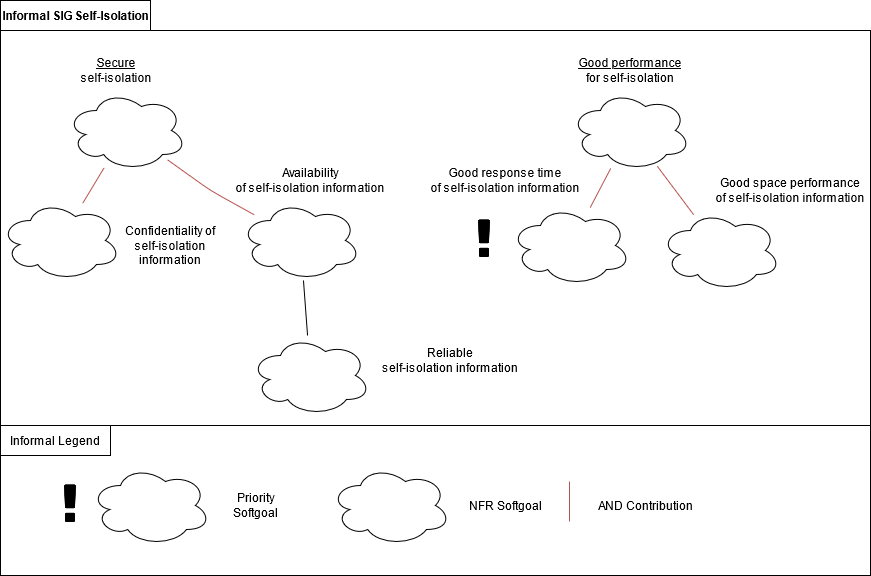
\includegraphics[scale=0.5]{img/Self-Isolation-2}
			\caption{Self Isolation - Decomposing NFRs} % Antraštė įterpiama po paveikslėlio
			\label{img:kurimoProcesas}
		\end{figure}
		

	\subsection{Infected patients}
		\begin{figure}[H]
			\center
			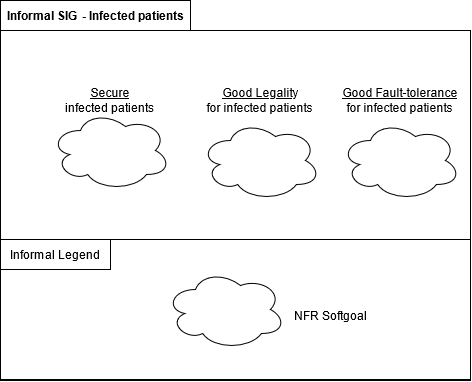
\includegraphics[scale=0.9]{img/Infected-Patients-1}
			\caption{Infected Patients - Initial Software Dependency Graph} % Antraštė įterpiama po paveikslėlio
			\label{img:kurimoProcesas}
		\end{figure}
		\begin{figure}[H]
			\center
			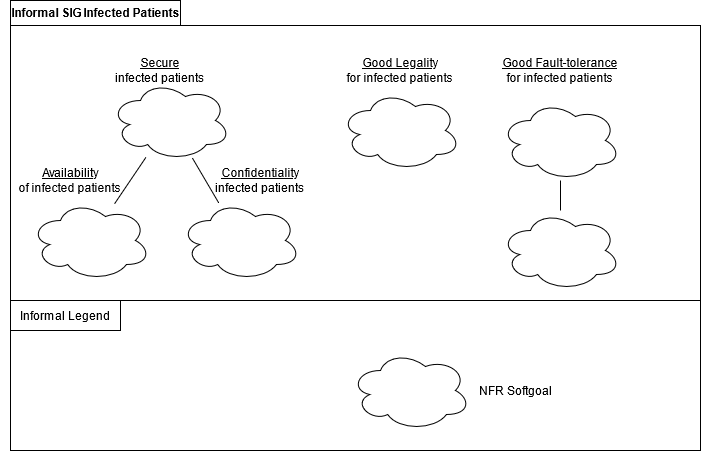
\includegraphics[scale=0.7]{img/Infected-Patients-2}
			\caption{Infected Patients - Decomposing NFRs} % Antraštė įterpiama po paveikslėlio
			\label{img:kurimoProcesas}
		\end{figure}



	\subsection{Dangerouse countries}
		\begin{figure}[H]
			\center
			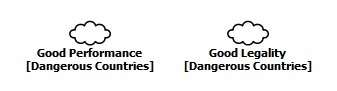
\includegraphics[scale=0.9]{img/Dangerous-Countries-1}
			\caption{Dangerous Countries - Initial Software Dependency Graph} % Antraštė įterpiama po paveikslėlio
			\label{img:kurimoProcesas}
		\end{figure}
		\begin{figure}[H]
			\center
			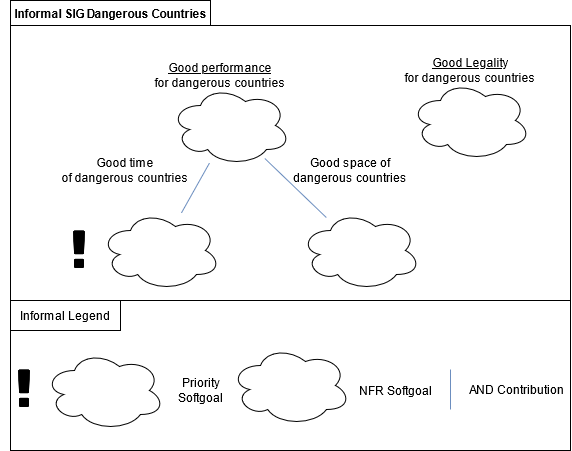
\includegraphics[scale=0.7]{img/Dangerous-Countries-2}
			\caption{Dangerous Countries - Decomposing NFRs} % Antraštė įterpiama po paveikslėlio
			\label{img:kurimoProcesas}
		\end{figure}	

\section{Identifying and modelling of possible operationalizations for NFR}
	\subsection{Self-isolation}
			\begin{figure}[H]
				\center
				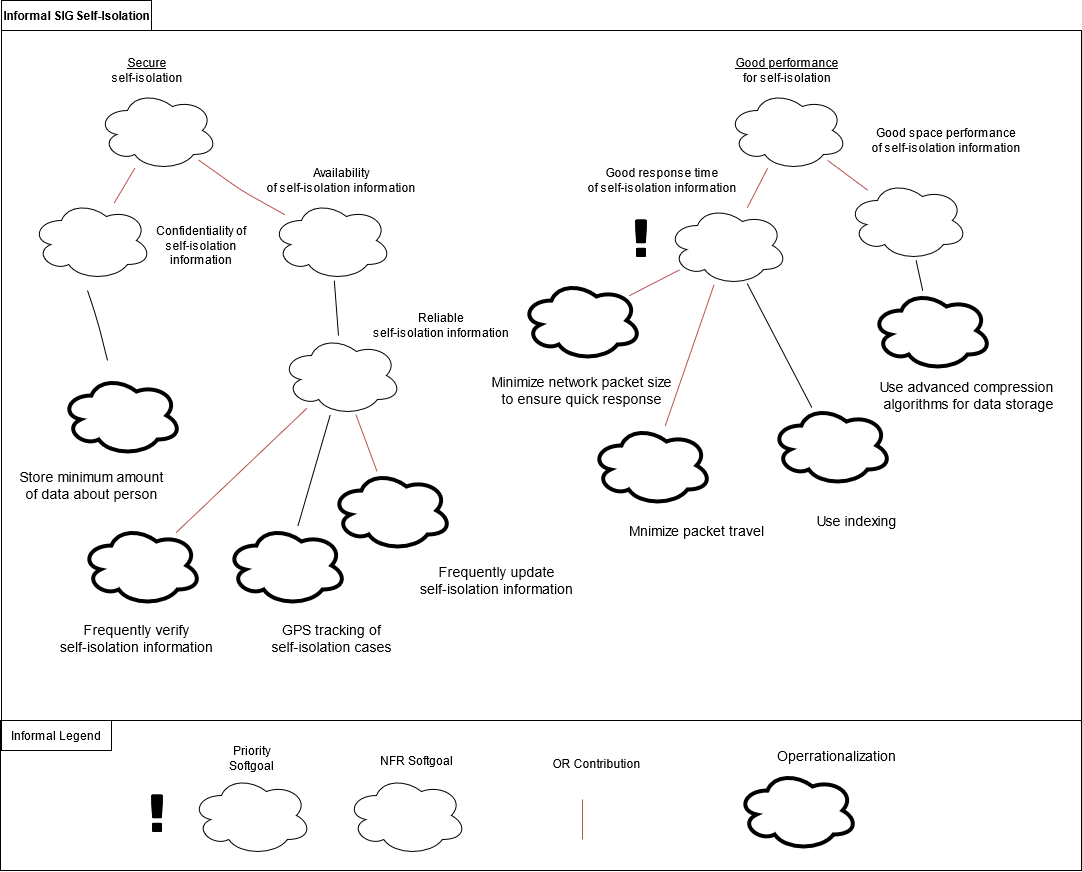
\includegraphics[scale=0.4]{img/Self-Isolation-3}
				\caption{Self Isolation - Possible Operationalizations} % Antraštė įterpiama po paveikslėlio
				\label{img:kurimoProcesas}
			\end{figure}
		
	\subsection{Infected patients}
		\begin{figure}[H]
			\center
			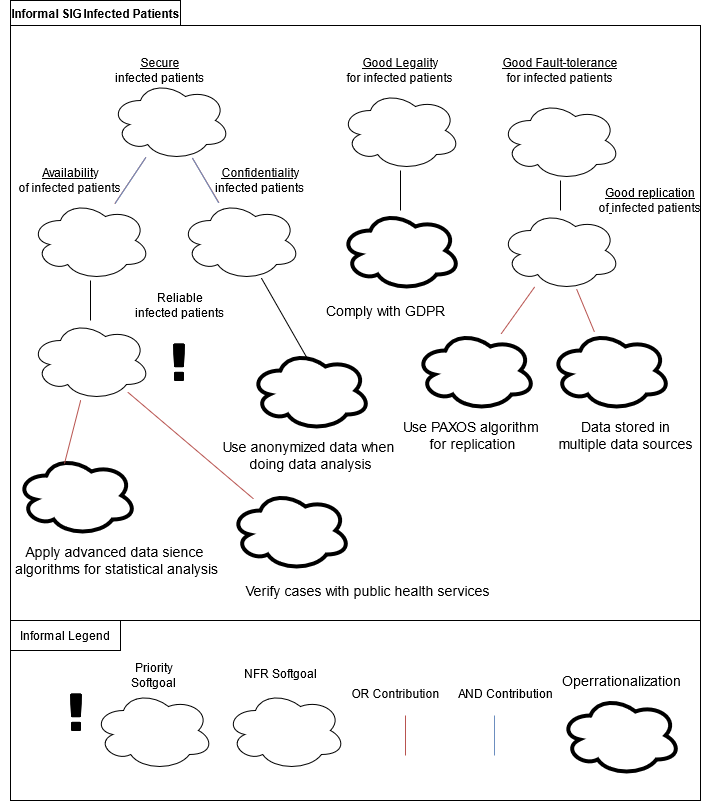
\includegraphics[scale=0.5]{img/Infected-Patients-3}
			\caption{Infected patients - Possible Operationalizations} % Antraštė įterpiama po paveikslėlio
			\label{img:kurimoProcesas}
		\end{figure}

	\subsection{Dangerouse countries}
		\begin{figure}[H]
			\center
			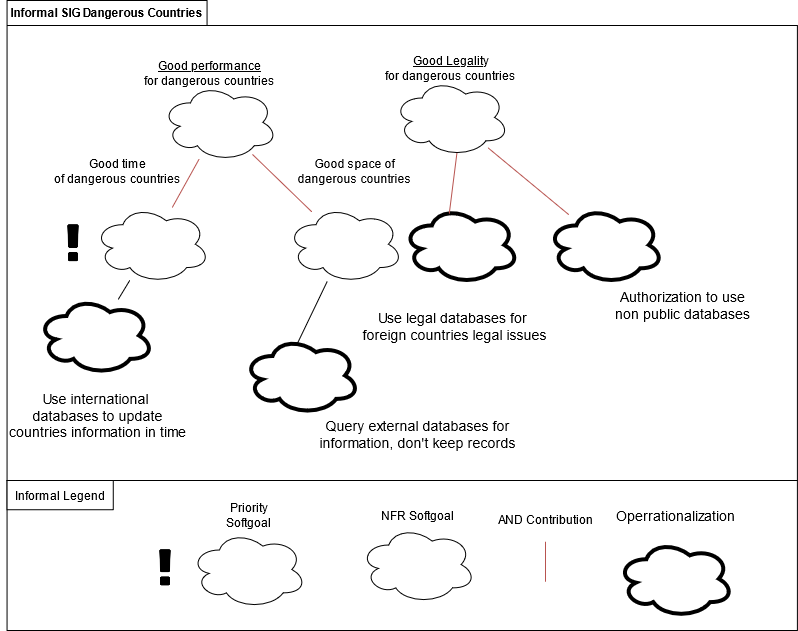
\includegraphics[scale=0.5]{img/Dangerous-Countries-3}
			\caption{Dangerous Countries - Possible Operationalizations} % Antraštė įterpiama po paveikslėlio
			\label{img:kurimoProcesas}
		\end{figure}	

\section{Detecting and Modelling of Implicit Interdependencies Among NFR}
	\begin{figure}[H]
		\center
		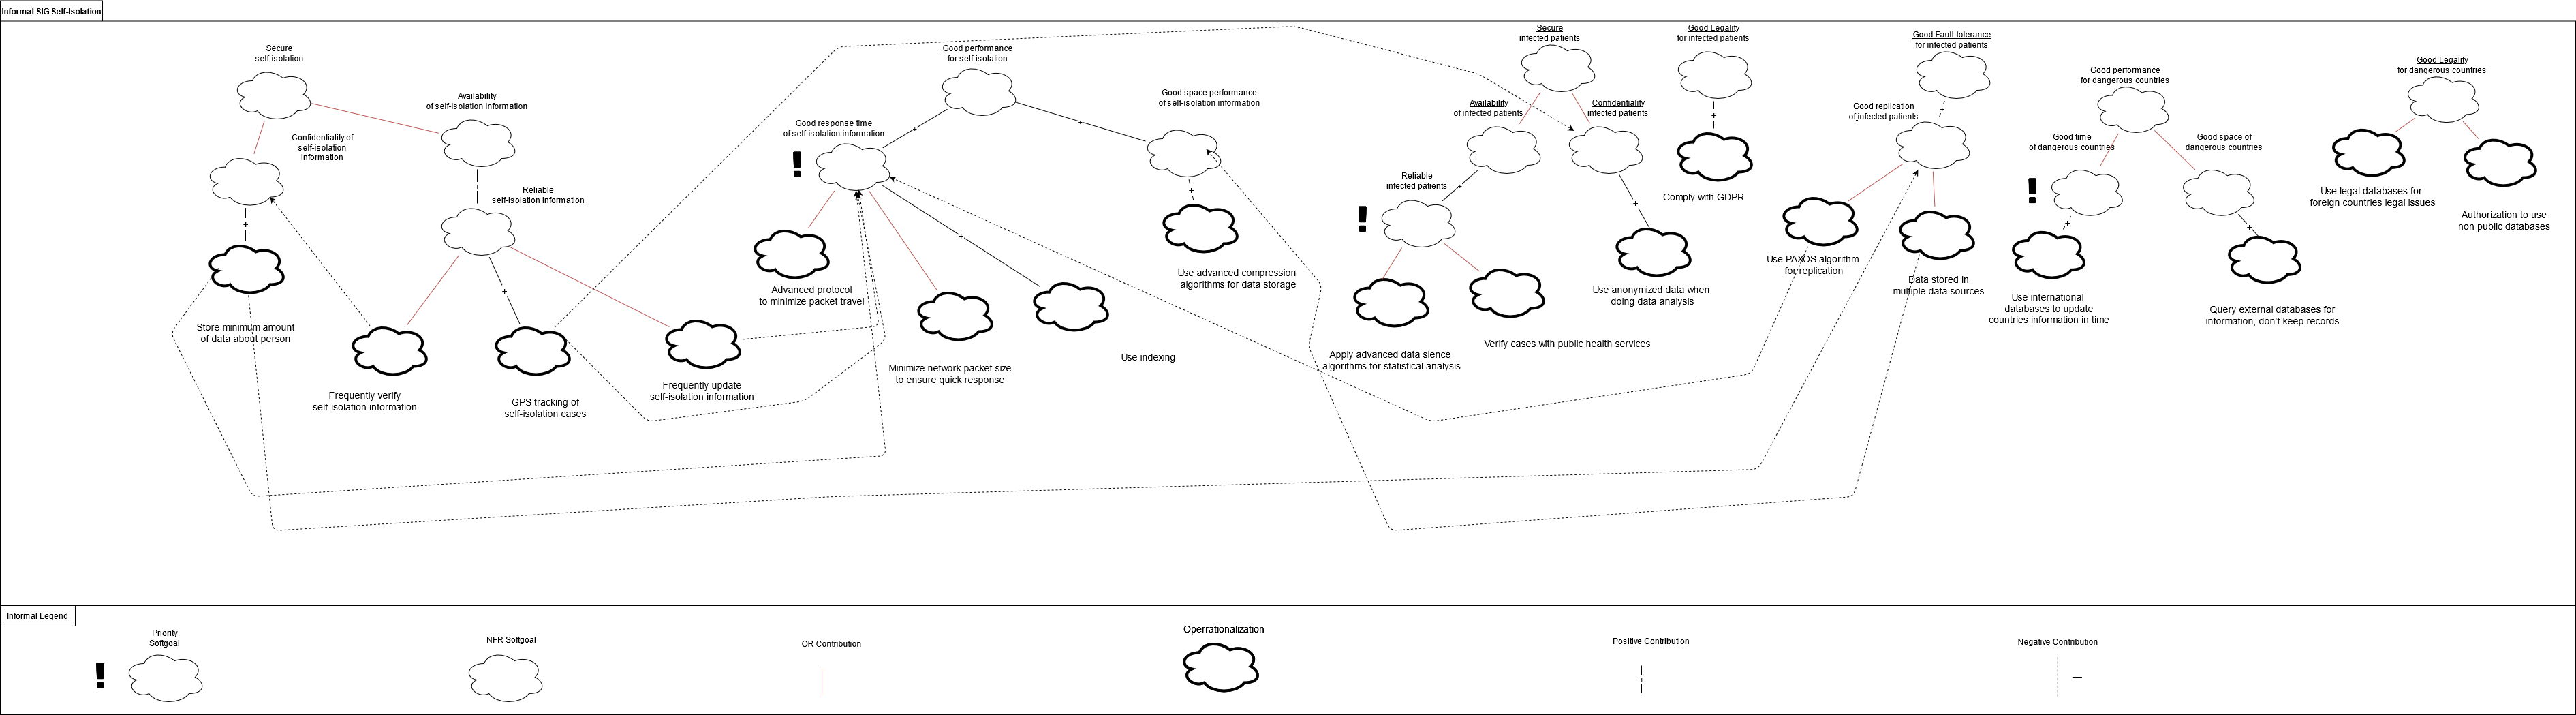
\includegraphics[scale=0.2]{img/Negative-Interdependancies}
		\caption{Implicit interdependencies among NFRs} % Antraštė įterpiama po paveikslėlio
		\label{img:kurimoProcesas}
	\end{figure}
\section{Making decisions}
\subsection{Chosen Operationalizations}
	\begin{figure}[H]
		\center
		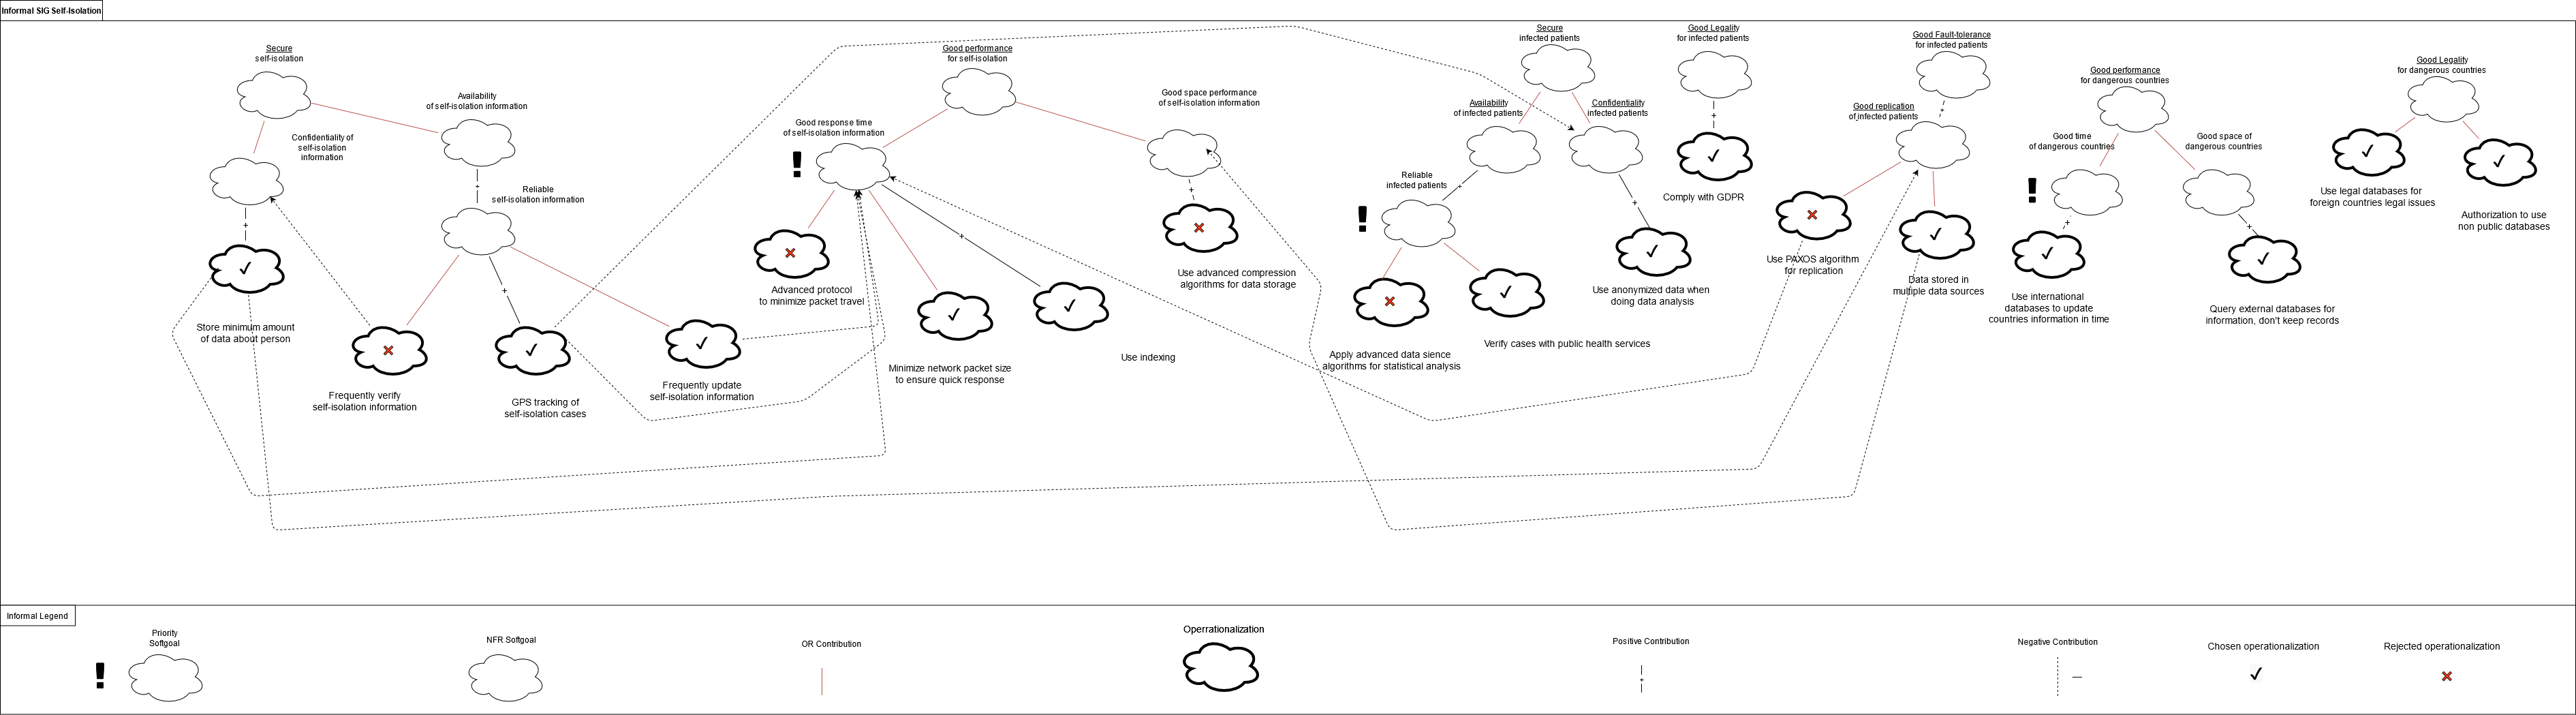
\includegraphics[scale=0.2]{img/Operationalization}
		\caption{Chosen Operationalizations among NFRs} % Antraštė įterpiama po paveikslėlio
		\label{img:kurimoProcesas}
	\end{figure}
	
	
\subsection{Chosen Softgoals}
	\begin{figure}[H]
		\center
		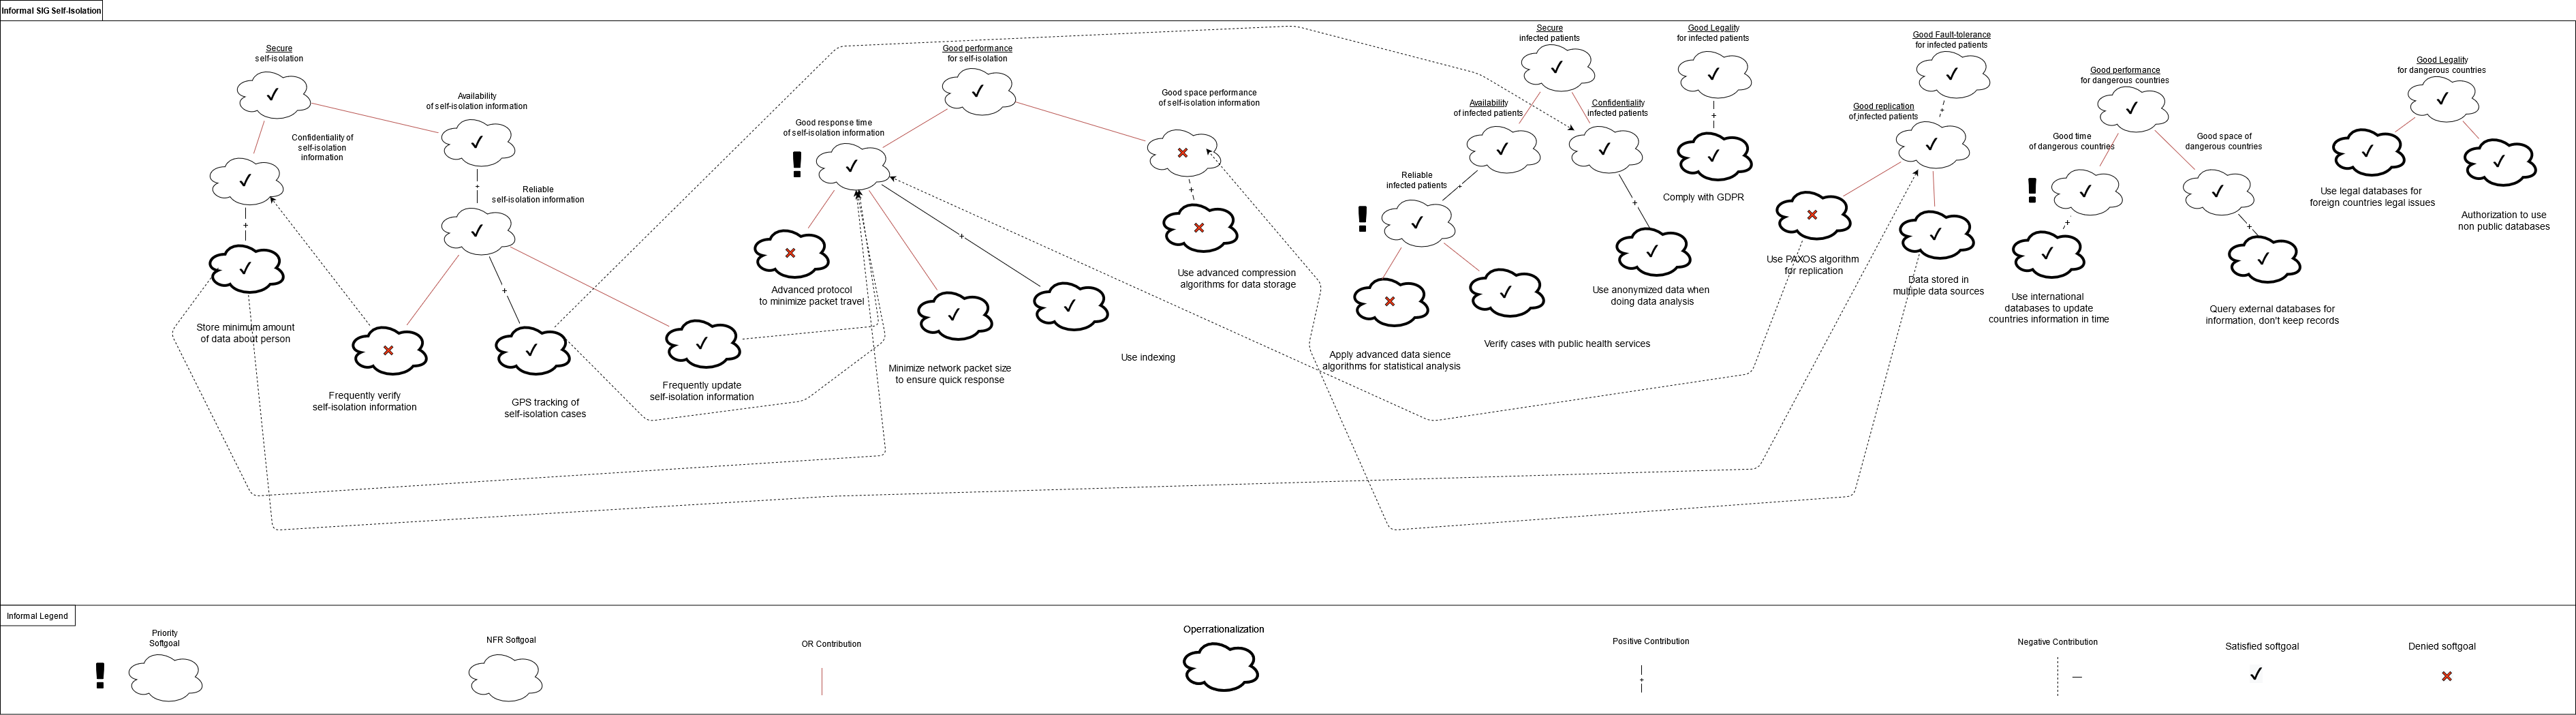
\includegraphics[scale=0.2]{img/Satisfied-Goals}
		\caption{Satisfied and Denied Softgoals} % Antraštė įterpiama po paveikslėlio
		\label{img:kurimoProcesas}
	\end{figure}
\end{landscape}
\subsection{Decision Explanation}
	\subsubsection{Negative impact}
		\begin{itemize}
			\item{Frequantly verify self-isolation information has negative impact on confitentiality because increasing amounts of data are processed with increases chance for data interception.}
			\item{Store minimum amount of data about person has negative impact on good respons time because querying small unstrctured data takes longer.}
			\item{Store minimum amount of data about person has negative impact on good replication because replication requires a lot of data to work properly.}
			\item{GPS tracking of self-isolation cases has negative impact on confidentiality because in case of data breach intruder might gain ability to know persons location.}
			\item{GPS tracking of self-isolation cases has negative impact on good response time because updating GPS information takes a long time.}
			\item{Frequently update self-isolation information has negative impact on response time because it takes computer resources to do the update.}
			\item{Use PAXOS algorithm for replication has negative impact on response time because this algorithm take a lot of computational resources to complete. Which impact respose time.}
			\item{Data stored in multiple data sources has negative impact on good space because it takes a lot of physical computer space to store in multiple sources.}
		\end{itemize}
	\subsubsection{Rejected operationalization}
		\begin{itemize}
			\item{Frequantly verify self-isolation information - verification usualy can be a complex process also it heavily impacts confidentiality, thats why we decided to reject.}
			\item{Advanced protocol to minimize packet travel - lack of competency in team to implement such protocols.}
			\item{Use advanced compression algorithms for data storage - lack of competency in team to implement such algorithms.}
			\item{Apply advanced data science algoritms for statistical analysis - lack of competency in team to implement such algorithms.}
			\item{Use PAXOS algorithm for replication - lack of competency in team to implement such protocols.}
		\end{itemize}
\subsection{Conclusions}
 Using NFR we succesfuly selected, decomposed and chose operationalized softgoald to be completed in our project.
Analysis was very useful and applicable in real life scenarions in industry.
\section{Strategic Dependency Model}
\section{Strategic Rationale Model}
\section{Conclusions about an dependency}
	
\sectionnonum{Conclusions}

\end{document}
